% !TeX root = ../main.tex

\chapter{Resultados e Discussões \label{chap:resultados}}

\section{Metodologia de avaliação dos resultados}

Com base na metodologia exposta apresentamos neste capítulo os resultados experimentais que obtivemos na análise dos descritores dimensão fractal multiescala, energia de dobramento multiescala e entropia  multiescala.

Uma avaliação comparativa dos resultados obtidos com os descritores \emph{NMBE} e \emph{DFM} é apresentada na subseção a seguir para em seguida apresentarmos os resultados obtidos com o descritor entropia multiescala.
{\color{red}

\section{\emph{Classificação de formas e sua relação com  a função objetivo}}

\section{\emph{Análise exploratória visual de agrupamentos}}

\section{\emph{Recuperação de imagens baseada em conteúdo - CBIR}}}

\section{Visualização dos dados}

\subsection{\emph{DFM}}

\begin{figure}
 \caption{\label{fig:dfm99} (a) Matriz-U para as formas da base Kimia99 representadas com o descritor dimensão fractal multiescala. (b) Silhouette média por classe aferida a partir do descritor}
  \centering
  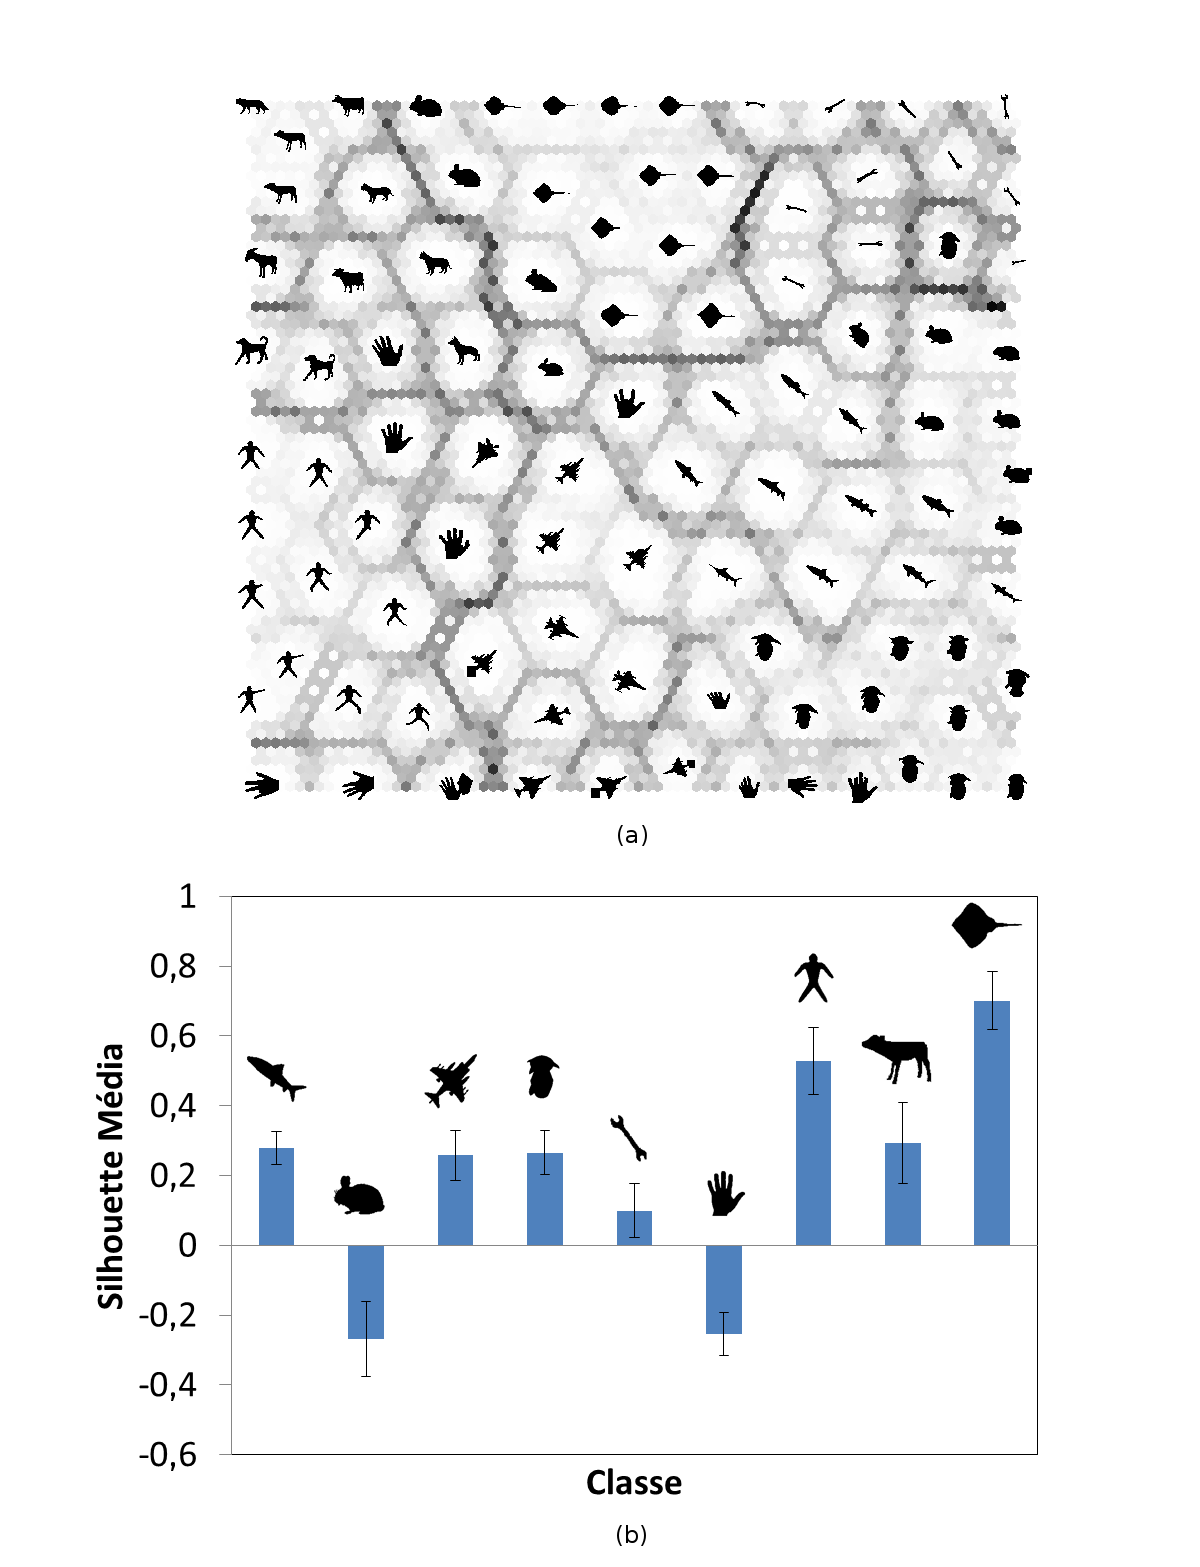
\includegraphics[width=\textwidth]{dfm99.png}
\end{figure}

\begin{figure}
 \caption{\label{fig:dfm216} (a) Matriz-U para as formas da base Kimia216 representadas com o descritor dimensão fractal multiescala. (b) Silhouette média por classe aferida a partir do descritor}
  \centering
  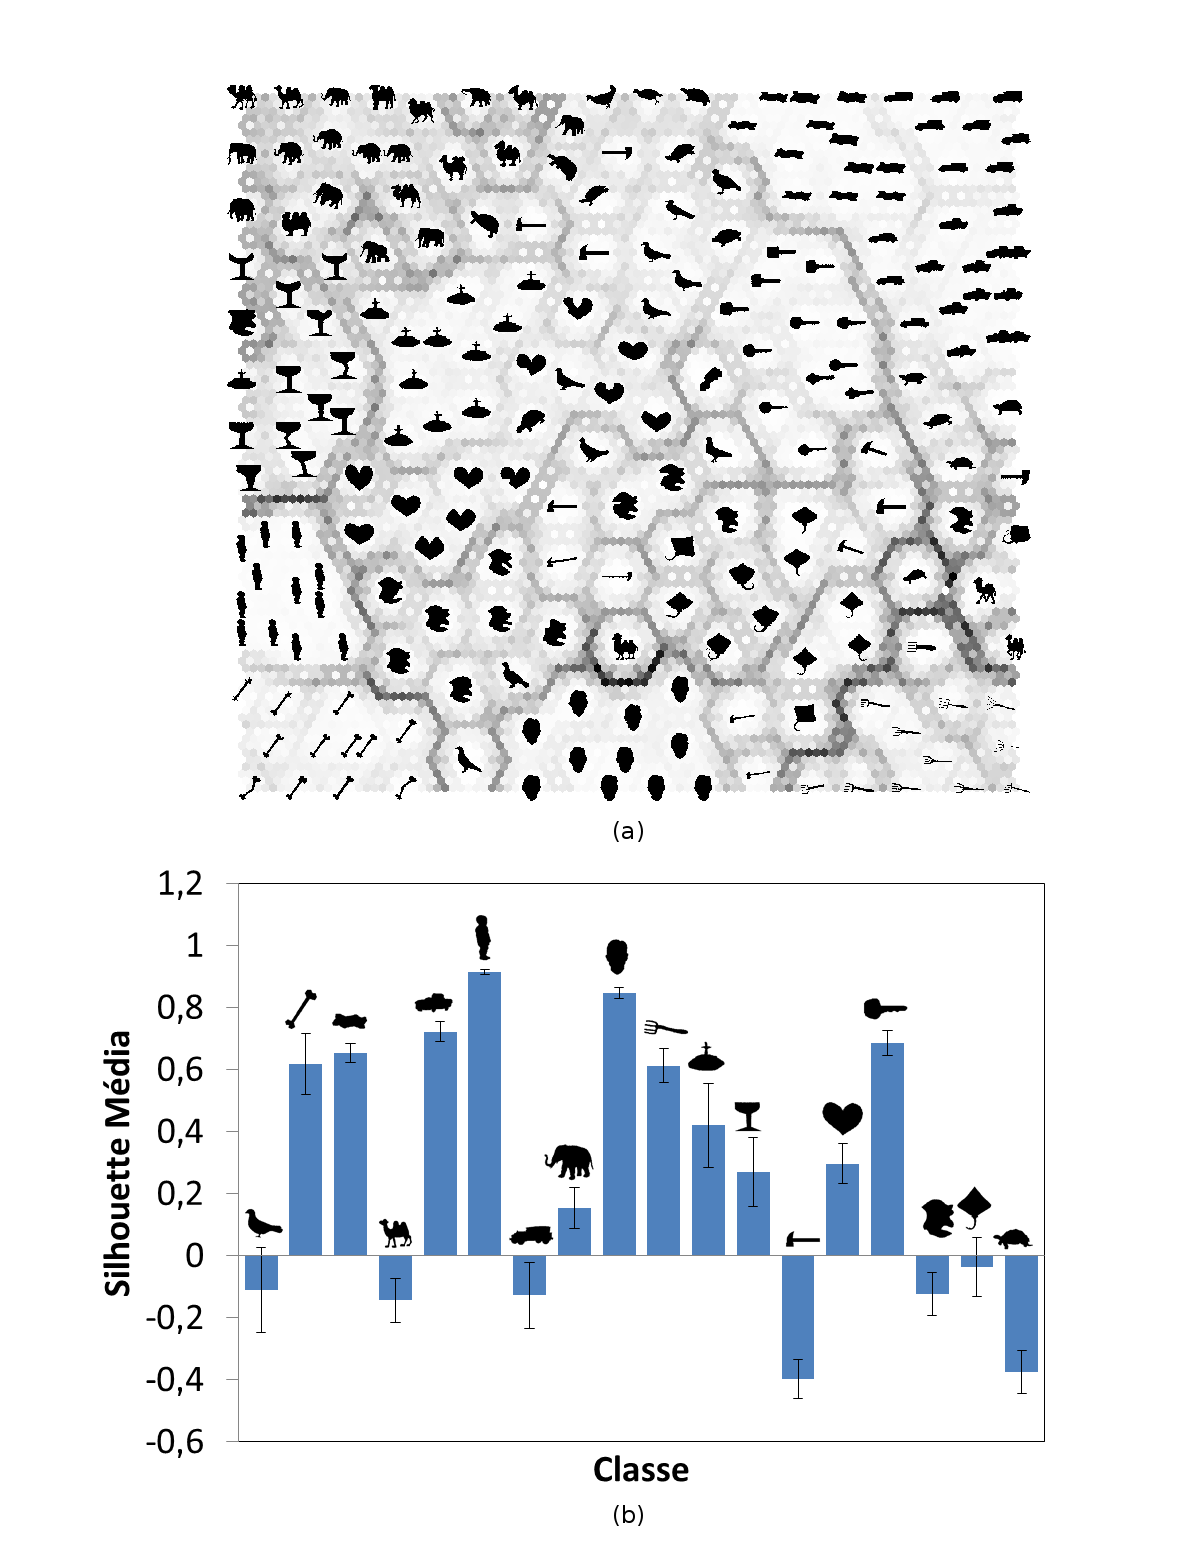
\includegraphics[width=\textwidth]{dfm216.png}
\end{figure}

\begin{figure}
 \caption{\label{fig:nmbe99} (a) Matriz-U para as formas da base Kimia99 representadas com o descritor energia de dobramento multiescala. (b) Silhouette média por classe aferida a partir do descritor}
  \centering
  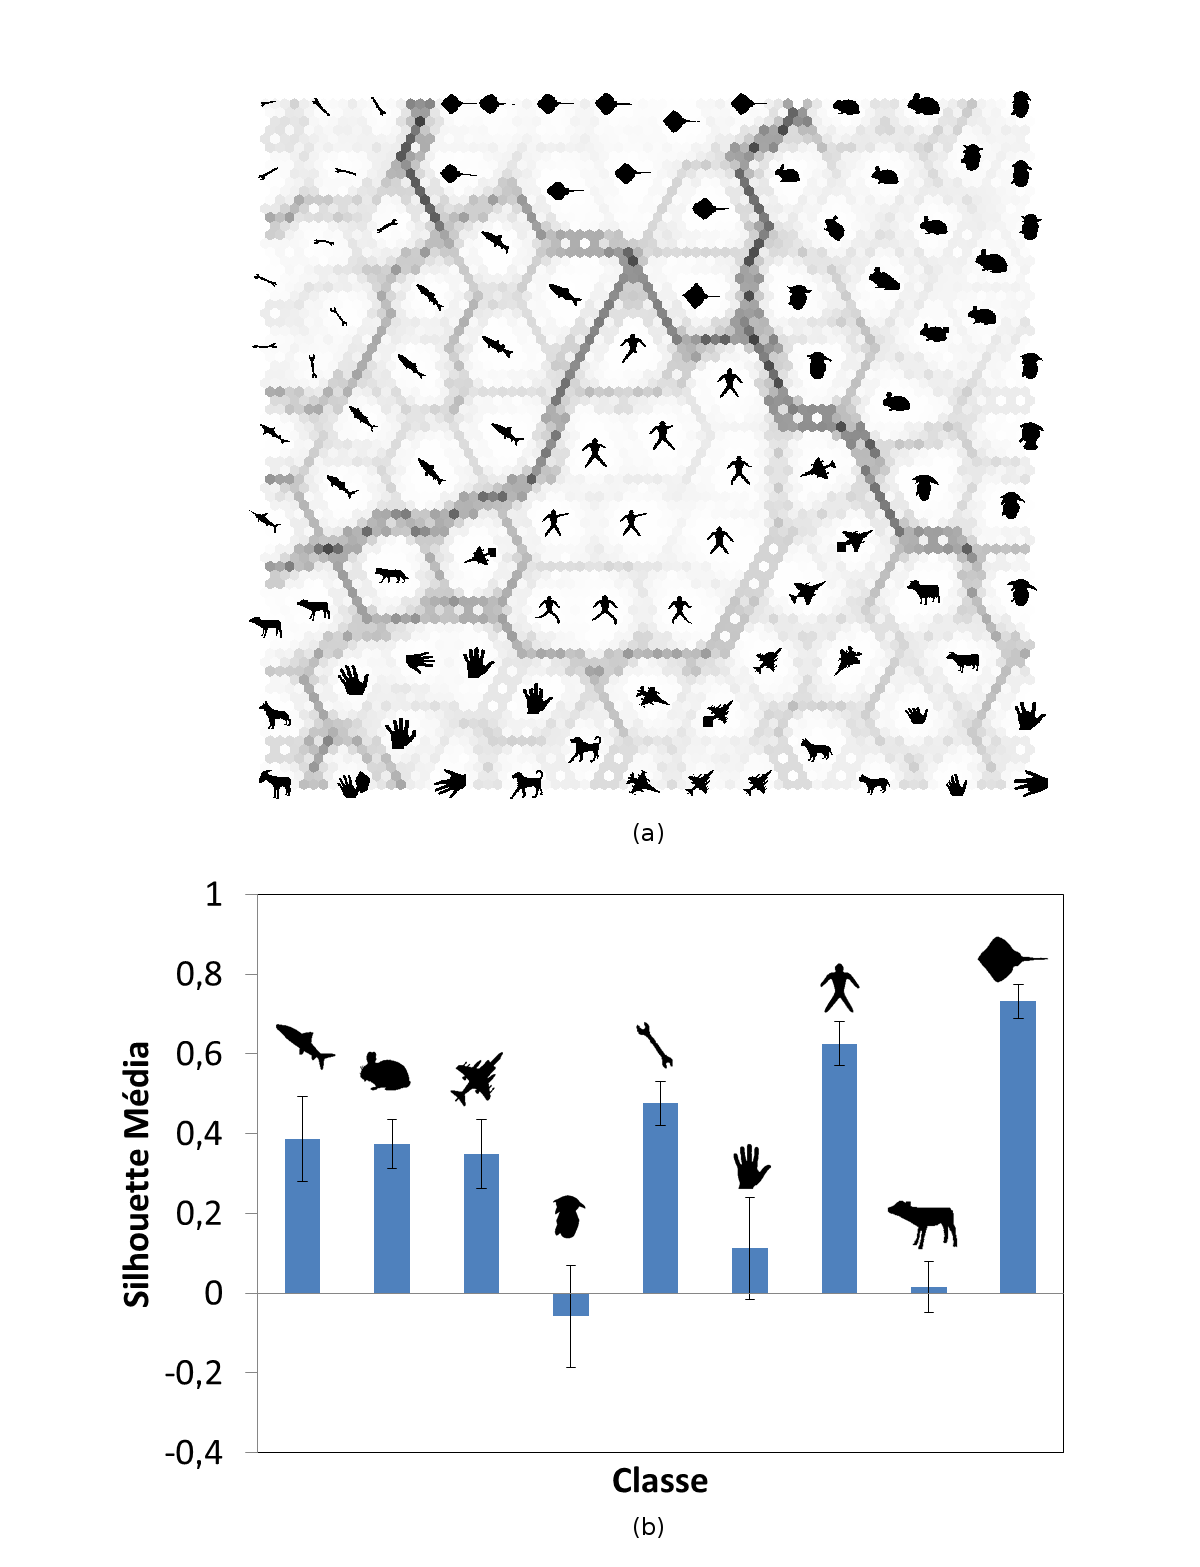
\includegraphics[width=\textwidth]{nmbe99.png}
\end{figure}

\begin{figure}
 \caption{\label{fig:nmbe216} (a) Matriz-U para as formas da base Kimia216 representadas com o descritor energia de dobramento multiescala. (b) Silhouette média por classe aferida a partir do descritor}
  \centering
  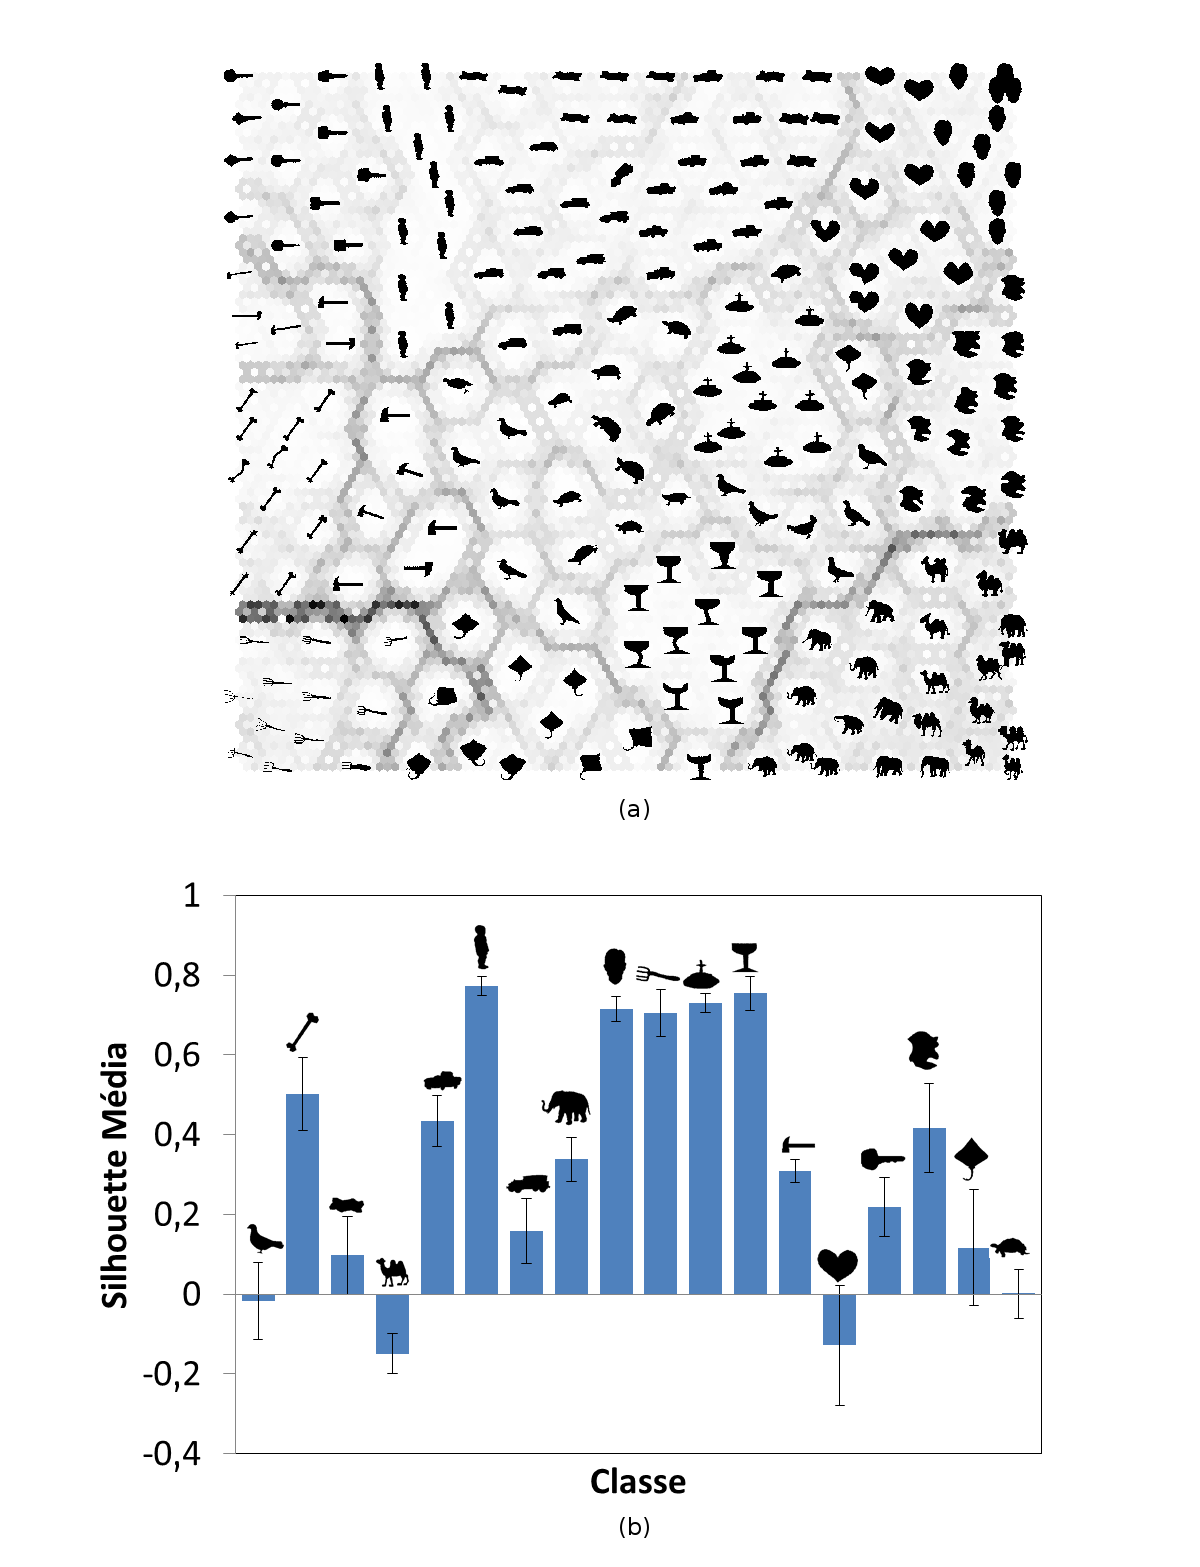
\includegraphics[width=\textwidth]{nmbe216.png}
\end{figure}

\begin{figure}
 \caption{\label{fig:edif99} (a) Matriz-U para as formas da base Kimia99 representadas com o descritor entropia multiescala. (b) Silhouette média por classe aferida a partir do descritor}
  \centering
  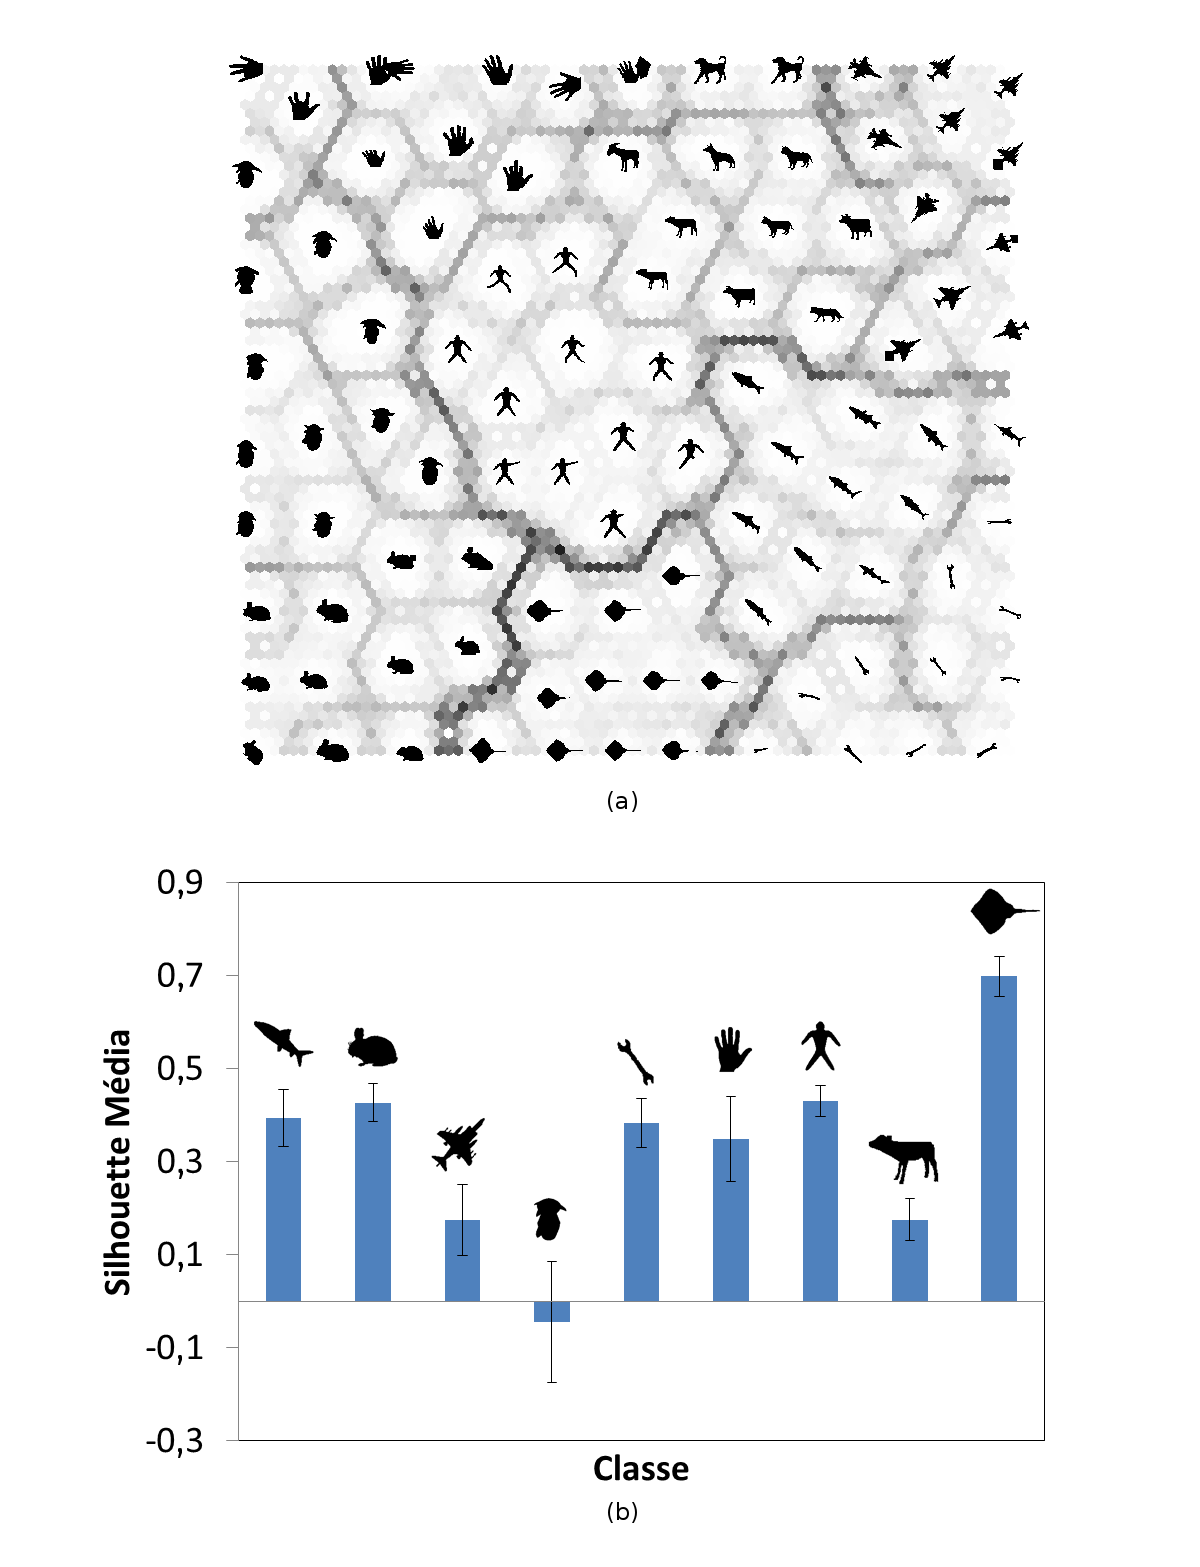
\includegraphics[width=\textwidth]{ediferencial99.png}
\end{figure}

\begin{figure}
 \caption{\label{fig:edif216} (a) Matriz-U para as formas da base Kimia216 representadas com o descritor entropia multiescala. (b) Silhouette média por classe aferida a partir do descritor}
  \centering
  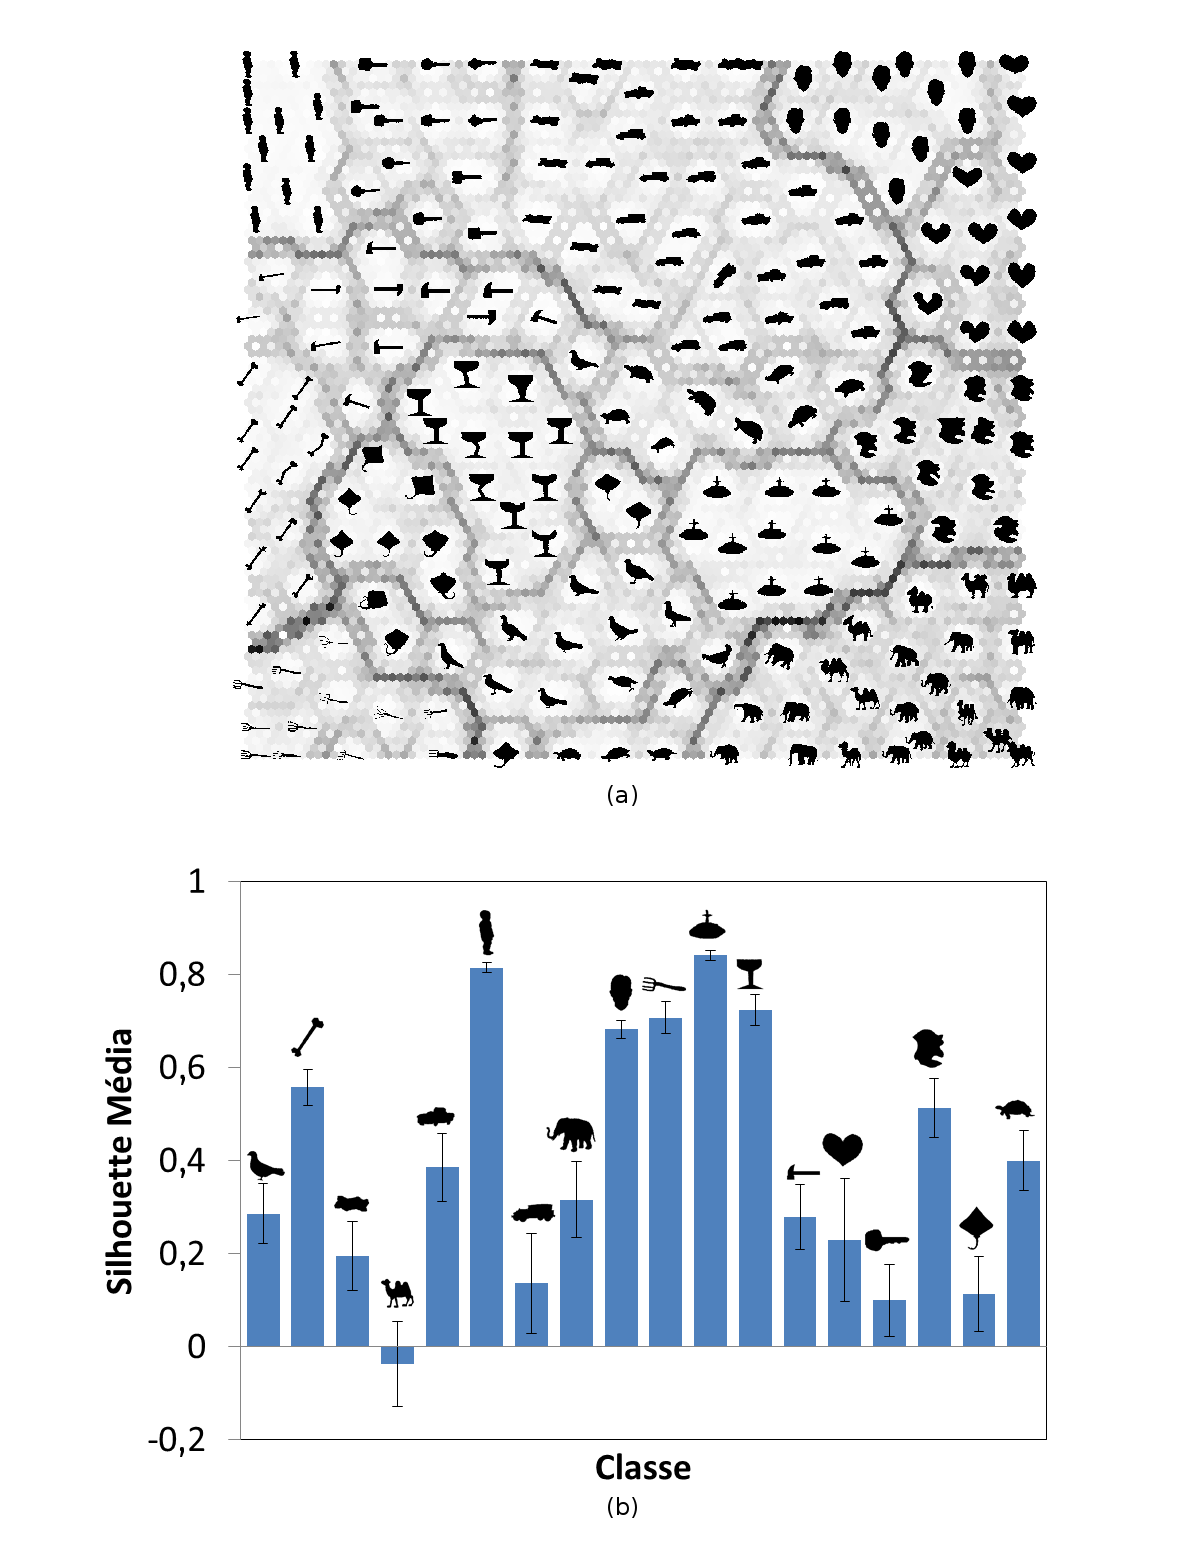
\includegraphics[width=\textwidth]{ediferencial216.png}
\end{figure}

\begin{figure}
 \caption{\label{fig:edis99} (a) Matriz-U para as formas da base Kimia99 representadas com o descritor entropia multiescala. (b) Silhouette média por classe aferida a partir do descritor}
  \centering
  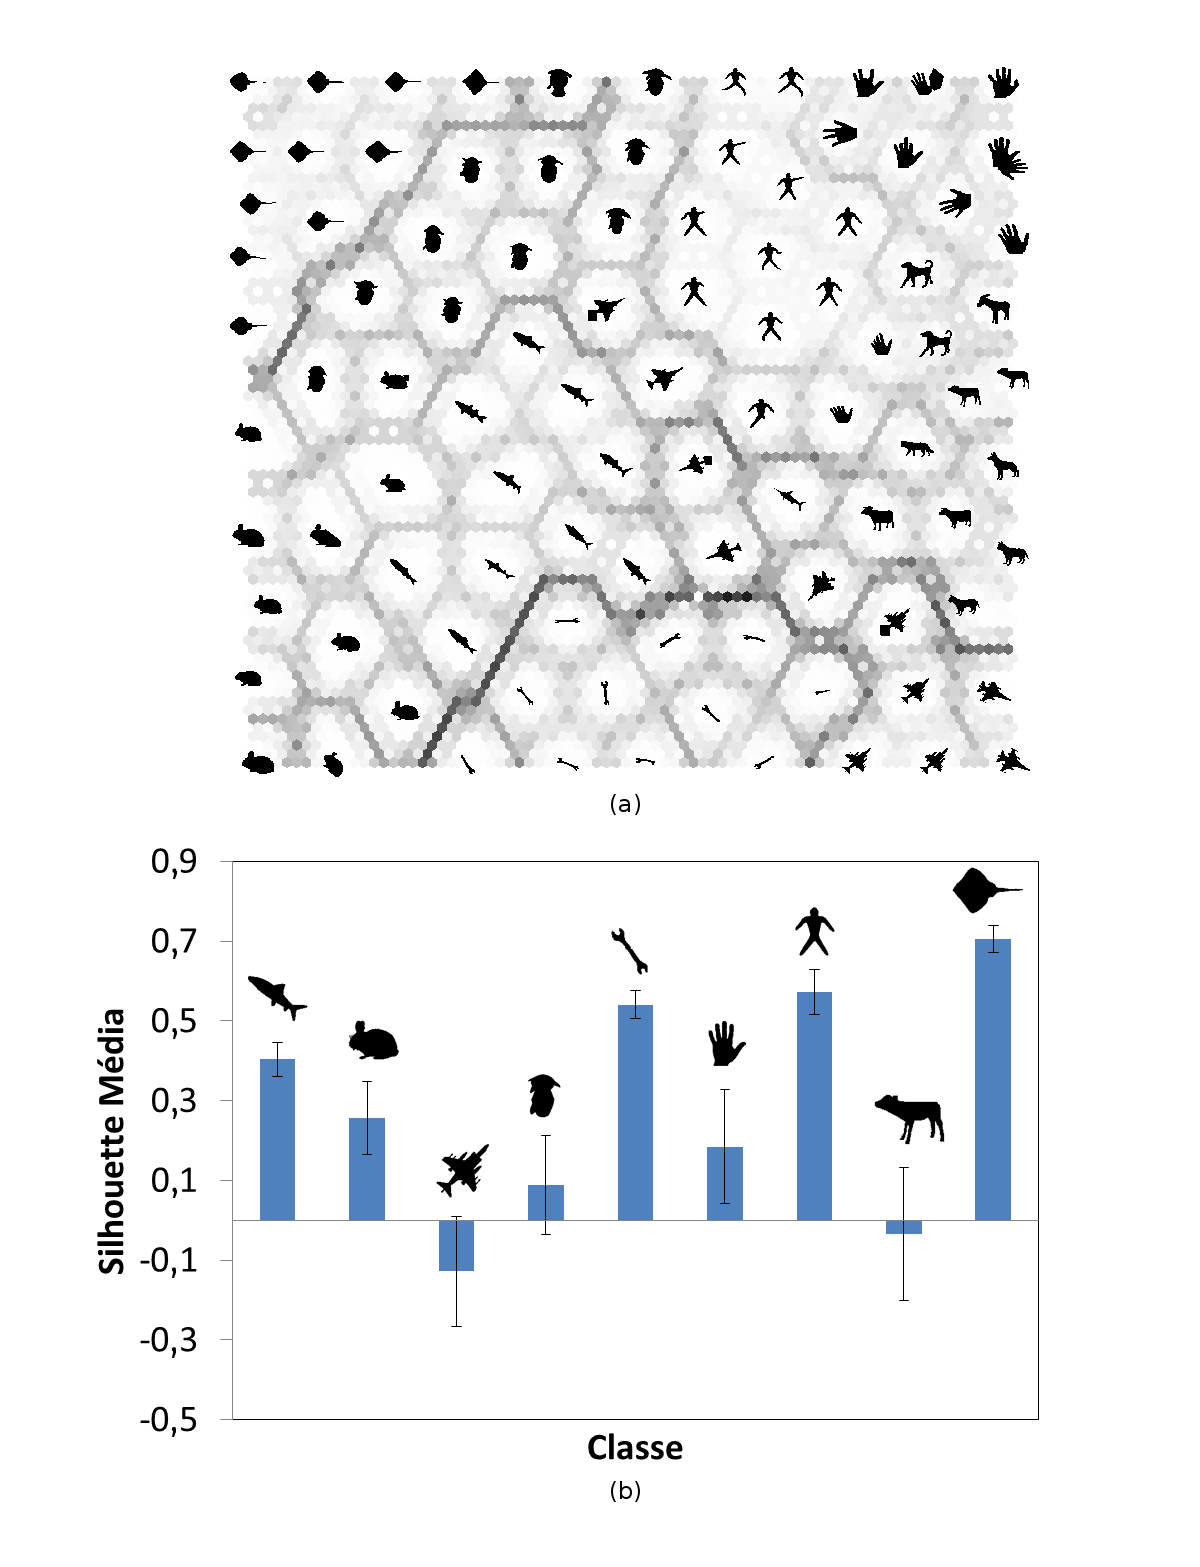
\includegraphics[width=\textwidth]{ediscreta99.png}
\end{figure}

\begin{figure}
 \caption{\label{fig:edis216} (a) Matriz-U para as formas da base Kimia216 representadas com o descritor entropia multiescala. (b) Silhouette média por classe aferida a partir do descritor}
  \centering
  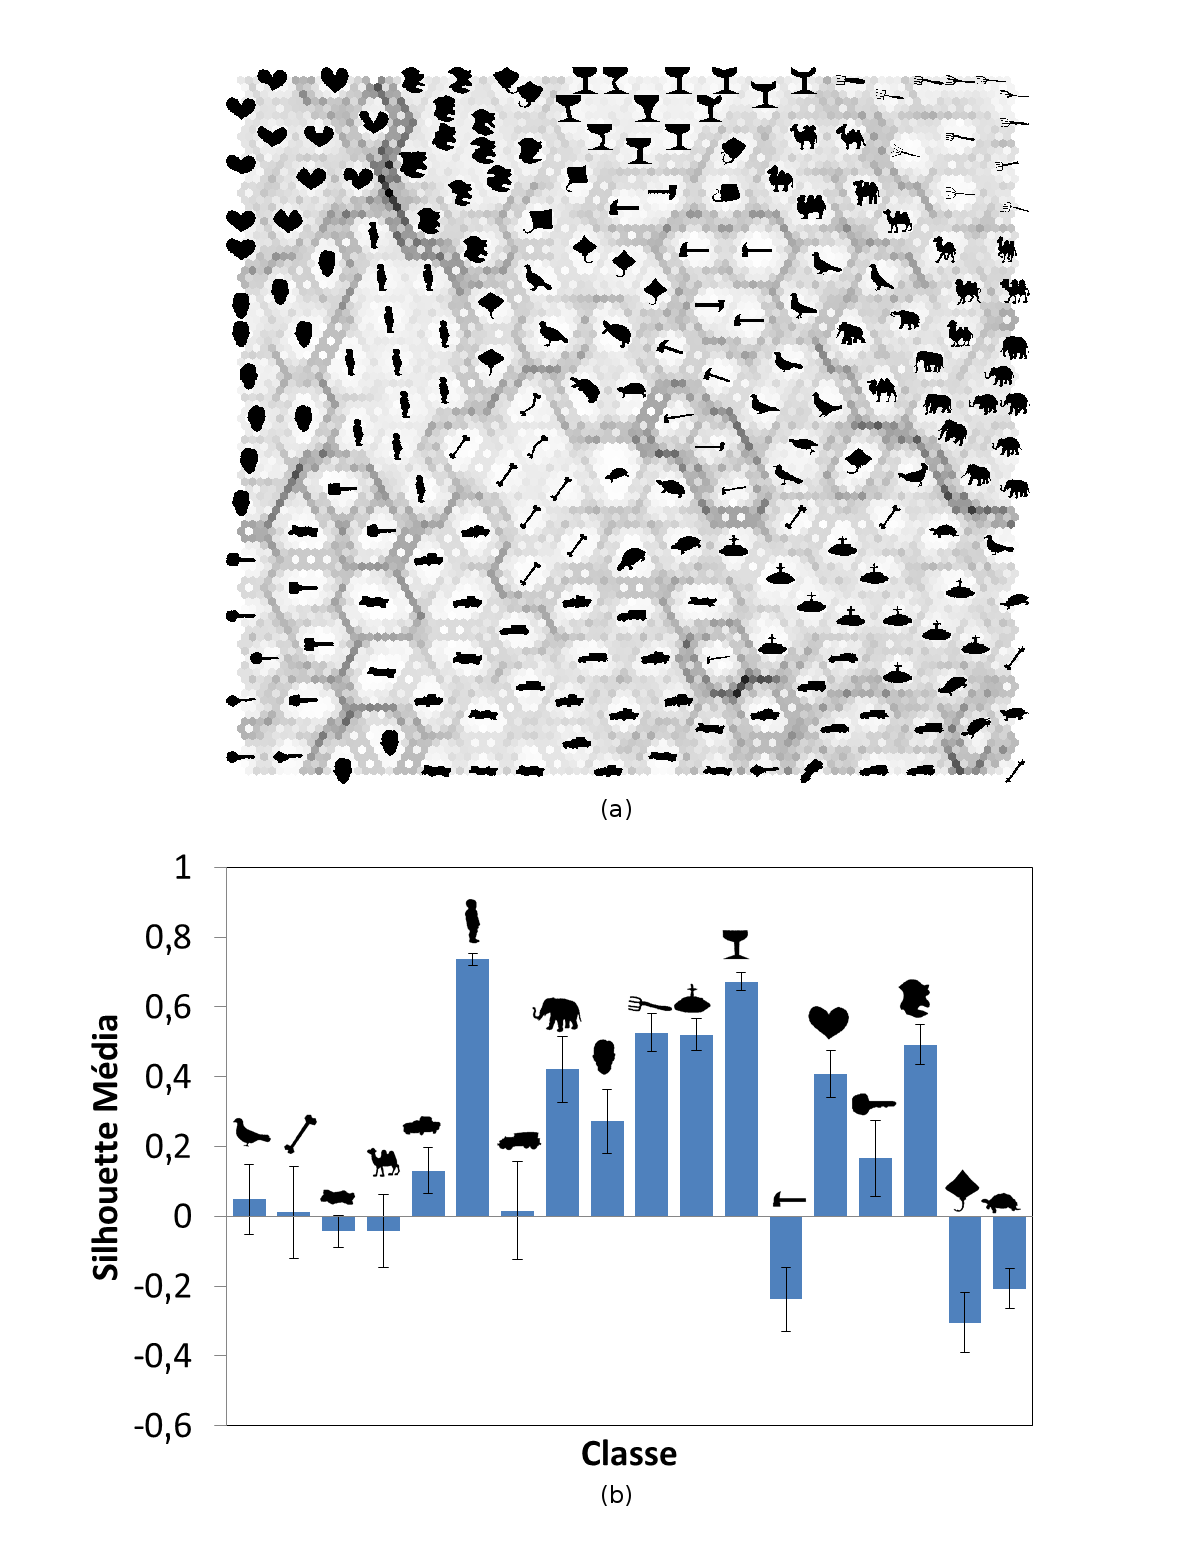
\includegraphics[width=\textwidth]{ediscreta216.png}
\end{figure}

\subsection{\emph{NMBE} e \emph{DFM}}
Os experimentos de avaliação de desempenho dos descritores produziram como saída as matrizes-U que estão apresentadas na Figuras \ref{fig:nmbe_som_map}, \ref{fig:mfd_som_map} e  \ref{fig:som_kimia_216}. Nas Figuras \ref{fig:nmbe_som_map} e \ref{fig:mfd_som_map}, as regiões delimitadas com linhas tracejadas correspondem as classes de formas com os maiores valores médios da medida Silhouette (Figuras \ref{fig:silhouette}a e \ref{fig:silhouette}b). Nesses casos pode-se deduzir que ambos os descritores foram capazes de caracterizar corretamente estas classes de formas.

Já os grupos delimitados com linhas contínuas referem-se às classes de formas com os menores valores de Silhouette média. De fato, as formas dessas classes aparecem nas matrizes-U dispersas em sub-grupos, que é um indicativo que ambos os descritores falharam em caracterizá-las adequadamente.
  
As Figuras \ref{fig:dude_tool_mfd} e \ref{fig:dude_tool_nmbe} mostram objetos das classes de formas de humanos e ferramentas. Ambos os descritores foram capazes de discriminar os objetos das referidas classes, como evidenciado nos gráficos apresentados. As matrizes-U (Figuras \ref{fig:nmbe_som_map} e \ref{fig:mfd_som_map}) também confirmam esse resultado exibindo, para essas classes de formas, homogeneidade intra-classe e separabilidade inter-classes. Logo, concluímos que estes descritores são efetivos em representar formas para o reconhecimento de padrões em aplicações \emph{CBIR}.

Também evidenciamos nas Figuras \ref{fig:mfd_som_map} e \ref{fig:nmbe_som_map} que o descritor \emph{DFM} apresentou maior dispersão inter-classe para as formas de humanos que o descritor \emph{NMBE}. Essa observação é consistente com os resultados obtidos através da medida \emph{Silhouete}, aonde o valor dessa medida para formas humanas descritas com a \emph{DFM} é menor do que o valor para essas mesmas formas descritas com a \emph{NMBE}.

Ademais, os sinais em linhas tracejadas vermelhas e em linhas contínuas azuis, apresentados nas Figuras \ref{fig:dude_tool_mfd} e \ref{fig:dude_tool_nmbe}, mostram que o descritor \emph{NMBE} é mais robusto a diferenças intra-classe que o descritor \emph{DFM}. Nesses gráficos, as formas pertencentes a mesma classe que o descritor representa seguindo um mesmo padrão apresentam-se próximas umas das outras na matriz-U, enquanto as formas que o descritor representa divergindo do padrão são mapeadas na matriz-U distantes dos grupo correspondente. Exemplos desta última condição são as formas humanas rotuladas como $2$ e $4$ nas Figuras \ref{fig:dude_tool_mfd} e \ref{fig:dude_tool_nmbe}.

\begin{comment}


Furthermore, there is a larger variation among tools descriptions in the graphs of  the figure \ref{fig:descritores}a than the  variations observed in the graphs of the figure \ref{fig:descritores}b. Coherently, the corresponding shapes appears in the U-matrix more dispersed  for the \emph{MFD} description than for the \emph{NMBE} description.
\end{comment}



\begin{figure}[h!]
  \caption{\label{fig:nmbe_som_map} Matriz-U para as formas da base Kimia99 representadas com o descritor Energia de dobramento multiescala.}
  \centering
  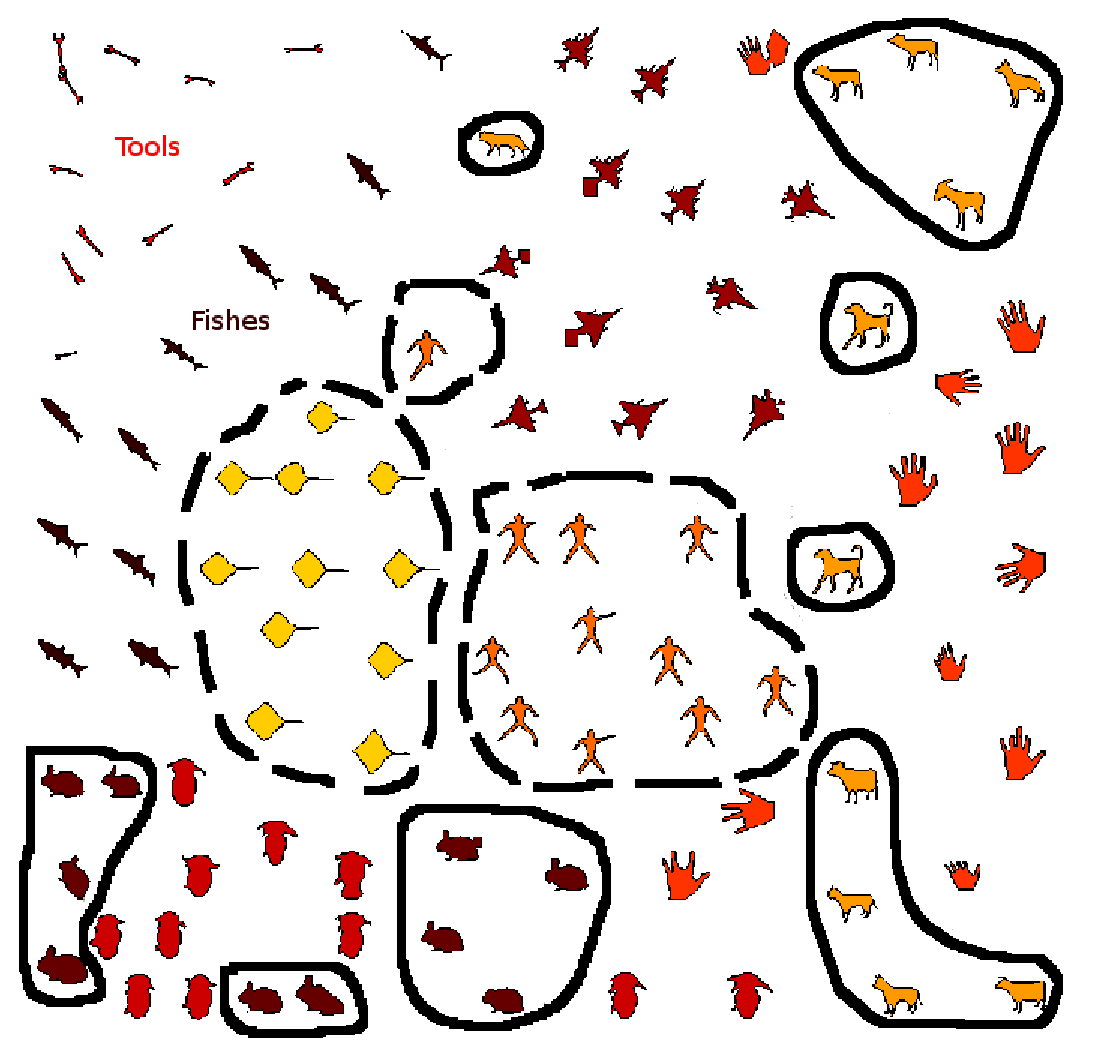
\includegraphics[width=0.5\textwidth]{nmbe_som_map_v4.eps}
\end{figure}

\begin{figure}[h!]
  \caption{\label{fig:mfd_som_map} Matriz-U para as formas da base Kimia99 representadas com o descritor Dimensão fractal multiescala.}
  \centering
  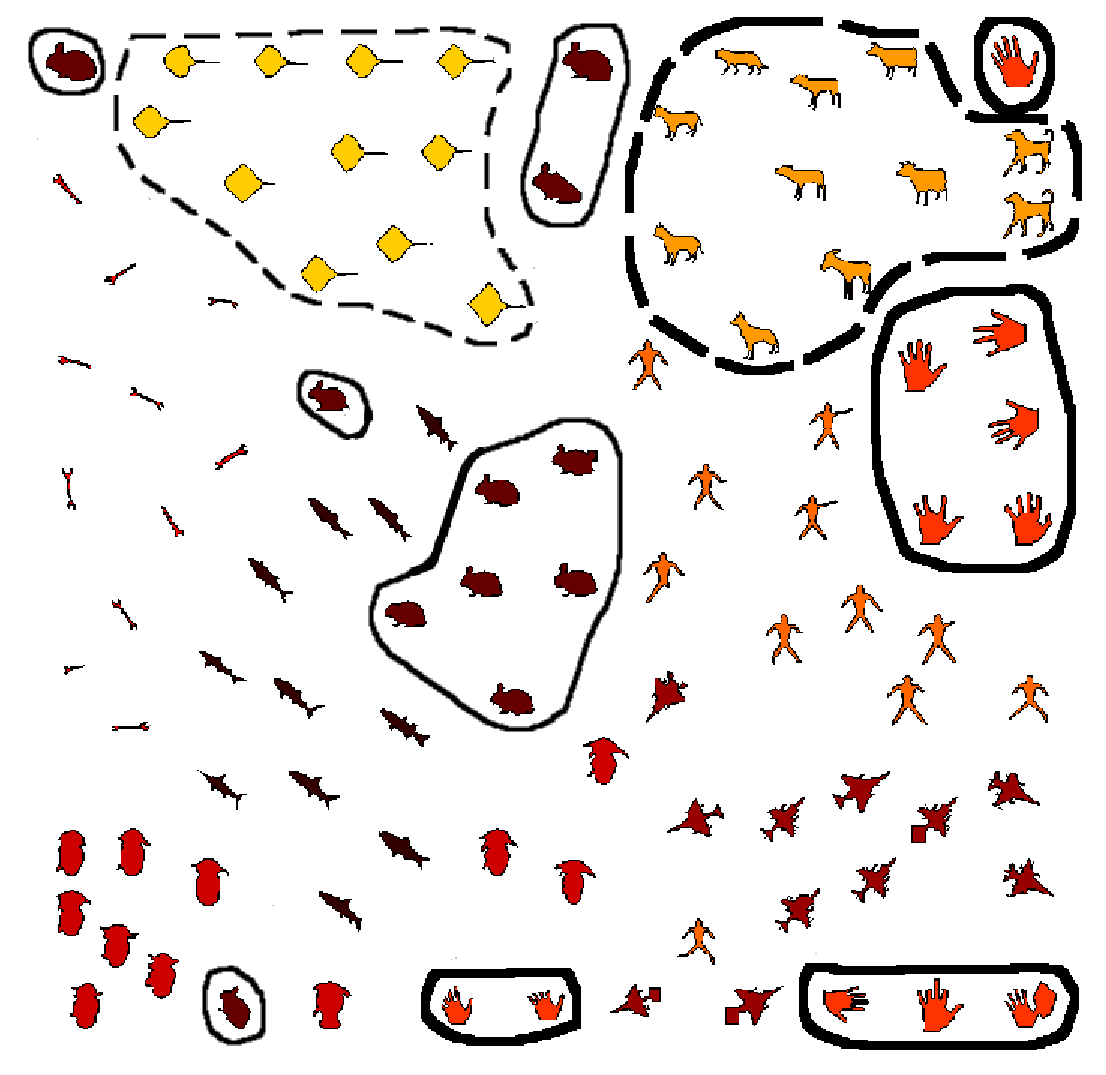
\includegraphics[width=0.5\textwidth]{mfd_som_map_v3.eps}
\end{figure}
  
\begin{figure}[h!]  \caption{\label{fig:som_kimia_216} Para o descritor energia de dobramento multiescala e a base Kimia-216: (a) Matriz-U. (b) Alguns resultados de recuperação de formas pelo conteúdo.}
  \centering
  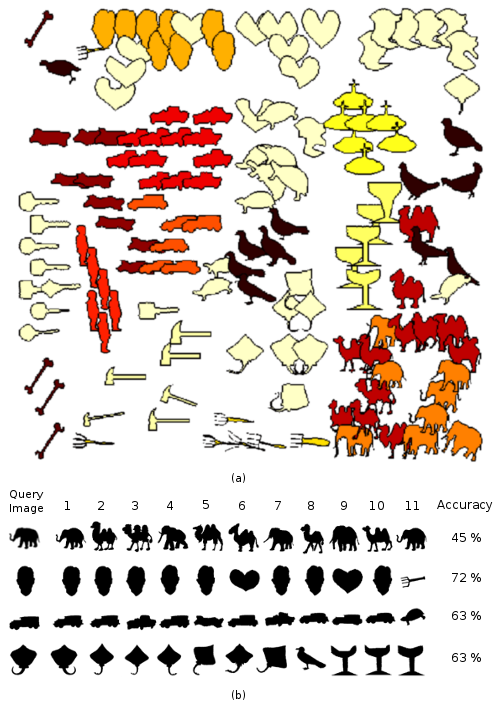
\includegraphics[width=0.5\textwidth]{retr_som_kimia216_v2.png}
\end{figure}

Já a Figura \ref{fig:som_kimia_216}a apresenta os resultados da visualização das formas da base Kimia-216 representadas através do descritor \emph{NMBE}. No canto inferior direito desta figura observamos que o descritor confunde formas dos elefantes com as dos camelos. Essa confusão aparece também no experimento de recuperação de formas pelo conteúdo (Figura \ref{fig:som_kimia_216}b), em que uma dentre as formas dos elefantes é utilizada como protótipo para se recuperar as onze formas mais similares ao protótipo na referida base.

Analogamente, no canto superior esquerdo da Figura \ref{fig:som_kimia_216}a, há confusão entre os agrupamentos das formas das faces e dos corações, bem como a presença duma forma de garfo. Na segunda linha da Figura \ref{fig:som_kimia_216}b observamos a presença dessas formas indesejáveis no experimento de recuperação de formas quando uma forma de face é apresentada como protótipo. 

Os demais resultados de recuperação de formas, apresentados na Figura \ref{fig:som_kimia_216}b, também estão coerentes com as observações da matriz-U. Nessa última podemos observar que o grupo das formas das arraias são mapeadas vizinhas aos grupos das formas dos cálices e dos pássaros, o que resulta no aparecimento das formas dessas últimas classes quando se realiza a recuperação de arraias. 

Outro aspecto importante de ser observado é que  grupos de formas com similaridades grosseiras encontram-se mapeados próximos uns dos outros na matriz-U. Formas alongadas, por exemplo, estão organizadas na parte inferior esquerda da Figura \ref{fig:som_kimia_216}a, enquanto formas arredondadas encontram-se na parte superior. Outros exemplos incluem os seguintes grupos: chaves e crianças (esquerda da figura), carros e tijolos, tartarugas e pássaros, cálices e sepulturas. 

\begin{figure}[h!]
  \caption{\label{fig:silhouette} Silhouette média por classe aferida, com a base Kimia-99, para os descritores (a) Dimensão fractal multiescala; (b) Energia de dobramento multiescala.}
  \centering
  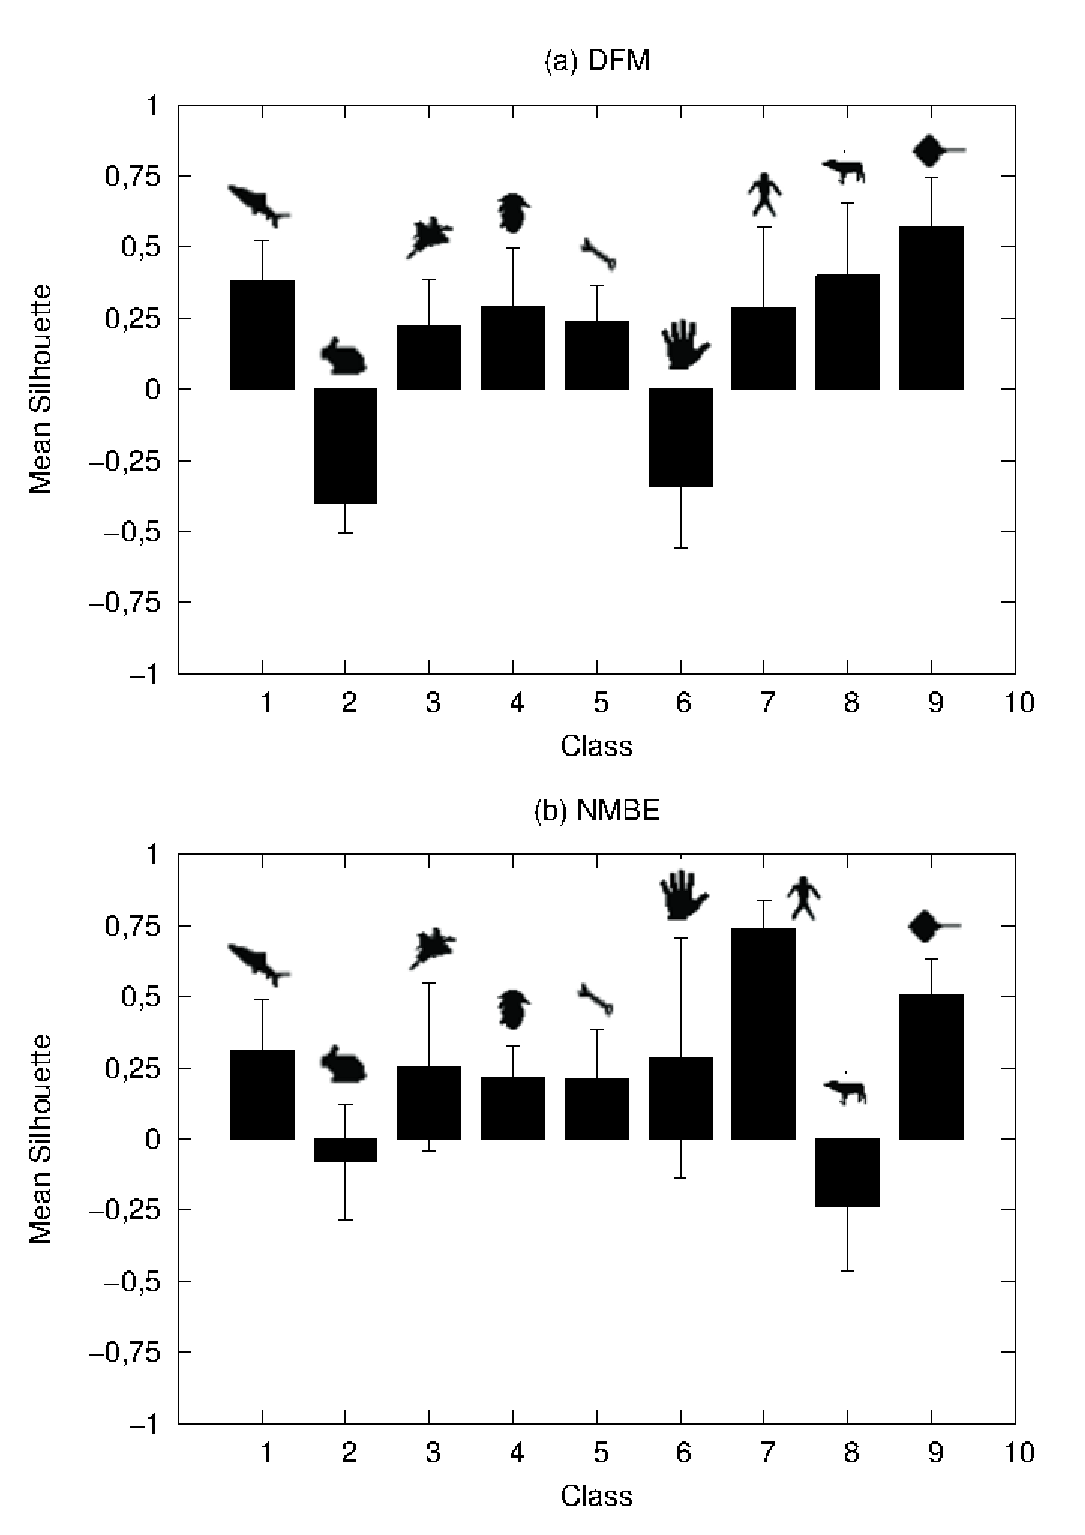
\includegraphics[width=0.5\textwidth]{resultado_silhouette.eps}
\end{figure}

\begin{figure}[h!]
  \caption{\label{fig:dude_tool_mfd}   Vetores de características calculados para amostras das formas de humanos e de ferramentas com o descritor dimensão fractal multiescala.}
  \centering
  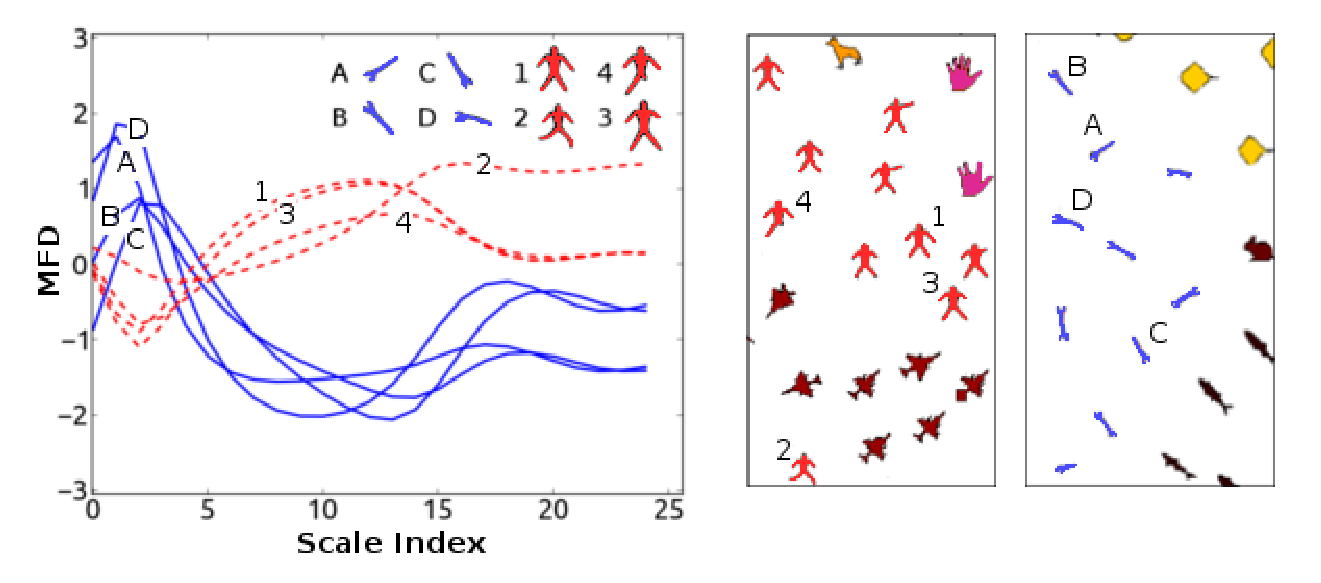
\includegraphics[width=0.75\textwidth]{dude_tool_mfd_v6.eps}
\end{figure}

\begin{figure}[h!]
  \caption{\label{fig:dude_tool_nmbe} Vetores de características calculados para amostras das formas de humanos e de ferramentes com o descritor energia de dobramento multiescala.}
  \centering
  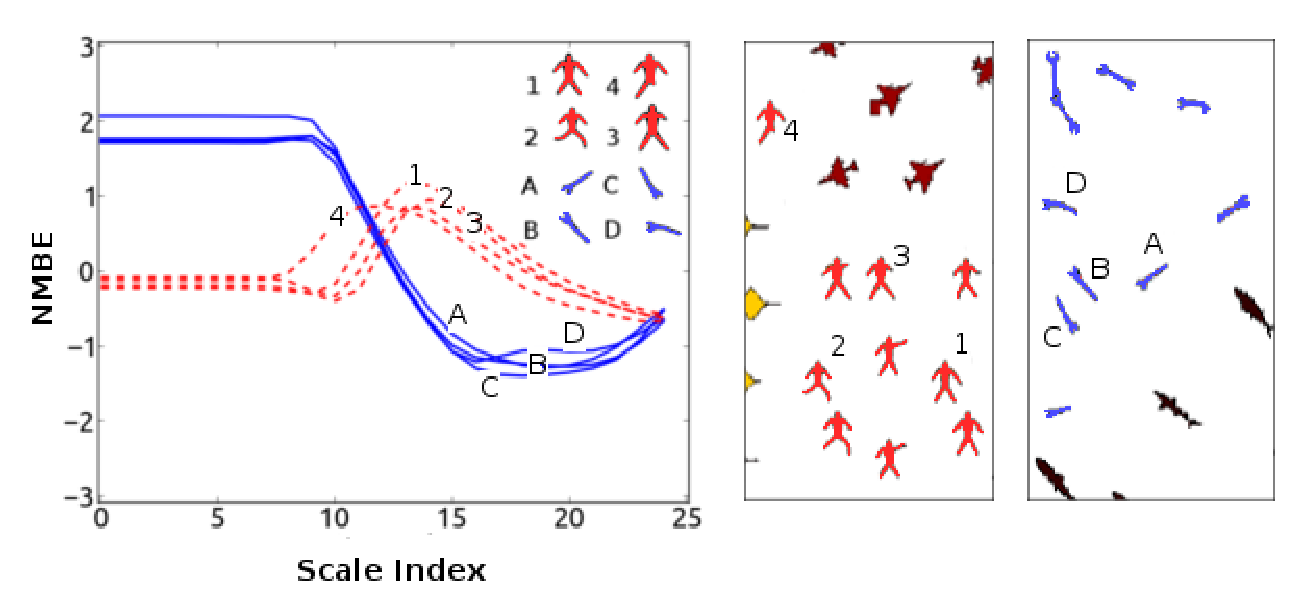
\includegraphics[width=0.75\textwidth]{dude_tool_nmbe_v6.eps}
\end{figure}

\subsection{Entropia diferencial da curvatura multiescala}

A visualização de dados obtida para características extraídas com o descritor entropia diferencial da curvatura multiescala, para a base Kimia-99, está apresentada na Figura \ref{fig:edif99}a. Nesta figura observamos a Matriz-U, em tons de cinza, sobreposta às figuras das formas nas posições mapeadas pela rede SOM.

As células escuras formam contornos que delimitam fronteiras existentes entre agrupamentos de formas, pois estas células indicam a existência duma relação de separação entre as formas em suas vizinhanças. Já as células em linhas claras indicam maior proximidade entre as formas e suas vizinhanças.

Podemos inferir que o descritor representou adequadamente as formas das classes de humanos, arraias, peixes, ferramentas e coelhos. Isso porque, nestes casos, o descritor apresentou uma representação compacta, agrupando próximas as formas de uma mesma classe, e propiciando separabilidade entre os agrupamentos estabelecidos. A medida Silhouette média por classe, apresentada na Figura \ref{fig:edif99}b, corrobora nossas observações, pois as referidas classes são as que apresentam os valores de Silhouette média mais positivos e com pequeno desvio padrão.  

Por outro lado, o descritor falhou em representar as formas das classes de animais quadrúpedes, aviões e extra terrestres. Isso porque, nesses casos, não se consegue identificar na matriz-U fronteiras claras que estabeleçam um único agrupamento das formas de uma mesma classe. Em outras palavras, formas dessas classes encontram-se separadas umas das outras ou dispersas em sub-grupos delimitados por pequenas fronteiras. Esses casos são os que apresentam a medida Silhouette média por classe com os menores valores e os maiores desvios padrão. 

Já na Figura \ref{fig:edif216}a temos a visualização da matriz-U para as características extraídas das formas da base Kimia-216. Nesta observamos, bem delimitados por linhas escuras, diversos agrupamentos  representados corretamente pelo descritor. Dentre esses, destacamos os agrupamentos cujas fronteiras de separação intra-classe são de baixo contraste e cujas fronteiras de separação inter-classe são bem contrastadas (faces, garfos, sepulturas, cálices e crianças). Esses são os  agrupamentos que apresentaram os maiores valores de \emph{Silhouette} média na Figura \ref{fig:edif216}b, o que é um resultado esperado, uma vez que o descritor representou as formas desses grupos de forma compacta e em agrupamentos bem separados.




\begin{comment}
\begin{figure}
\caption{\label{fig:edif_som_map} Matriz-U para as formas da base Kimia99 representadas com o descritor Entropia diferencial da curvatura multiescala.}
  \centering
  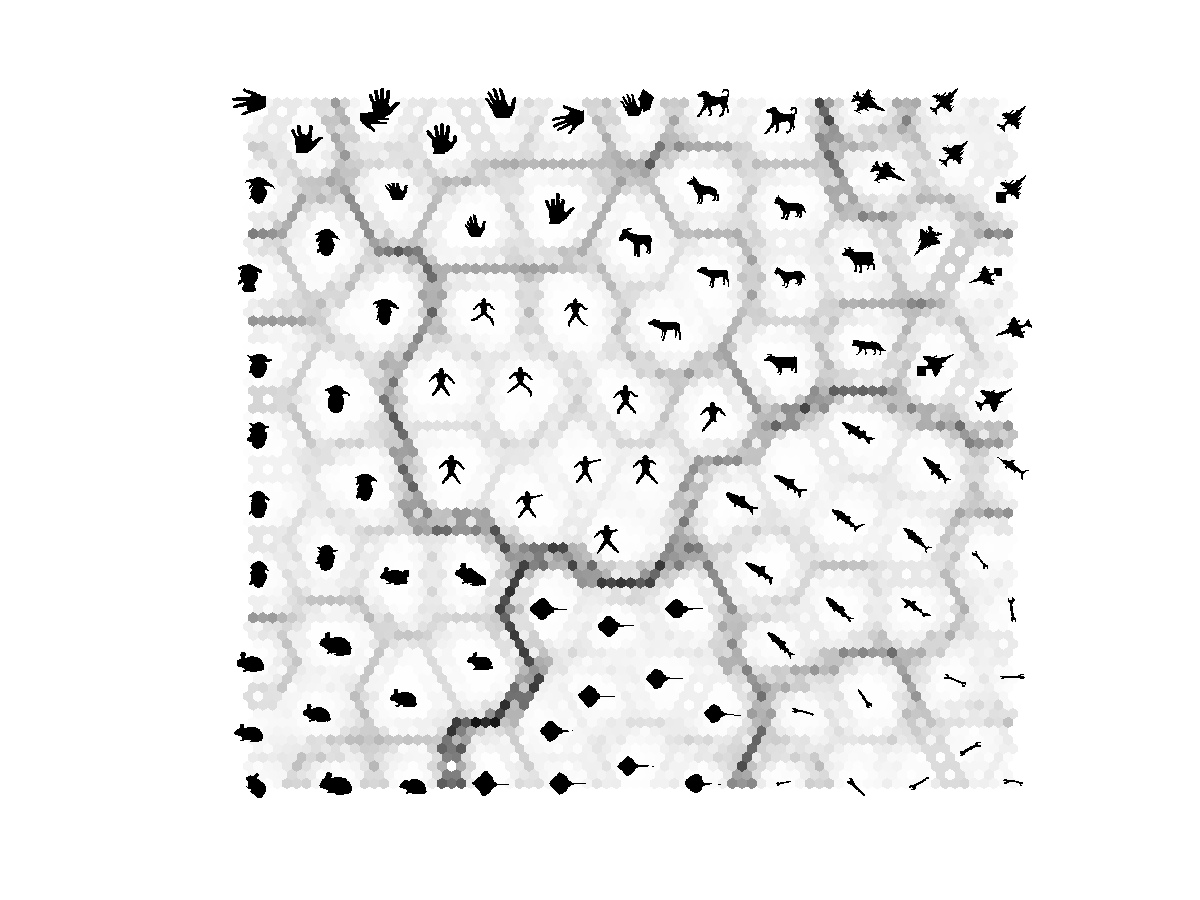
\includegraphics[width=\textwidth]{ediferencial_N5_formas.png}
 \end{figure}

\begin{figure}
\caption{\label{fig:silhouette_ediferencial} Silhouette média por classe aferida, com a base Kimia-99, para o descritor entropia diferencial da curvatura multiescala.}
  \centering
  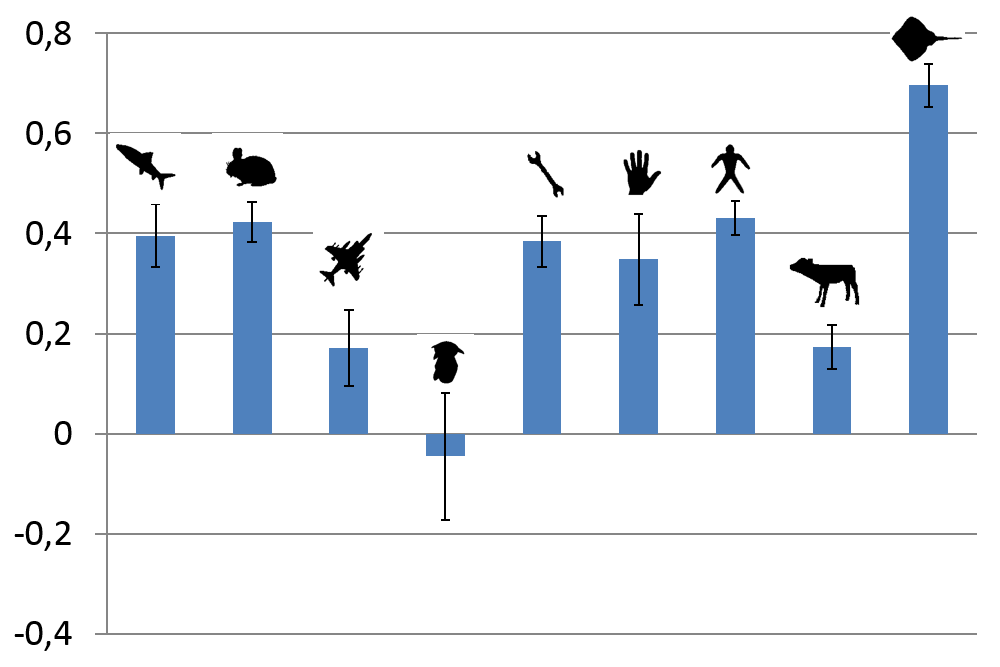
\includegraphics[width=0.75\textwidth]{ediferencial_silhouette_N5.png}
\end{figure}
\end{comment}

\begin{comment}
\begin{figure}[h!]
  \caption{\label{fig:som_nmbe} Visualização dos dados obtida com o mapa auto-organizável de Kohonen para a descrição \emph{NMBE}.}
  \centering
  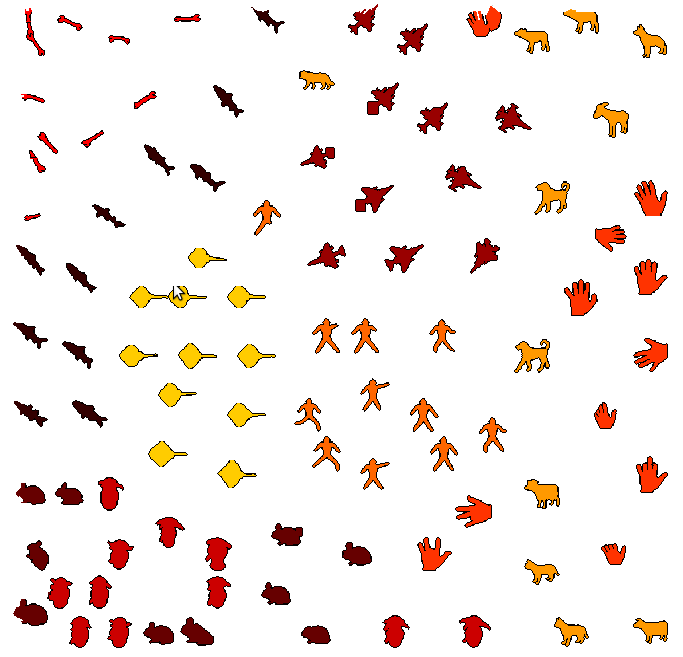
\includegraphics[width=0.5\textwidth]{mapa_som_descritor_nmbe.png}
\end{figure}

\begin{figure}[h!]
  \caption{\label{fig:som_dfm} Visualização dos dados obtida com o mapa auto-organizável de Kohonen para a descrição \emph{NMBE}.}
  \centering
  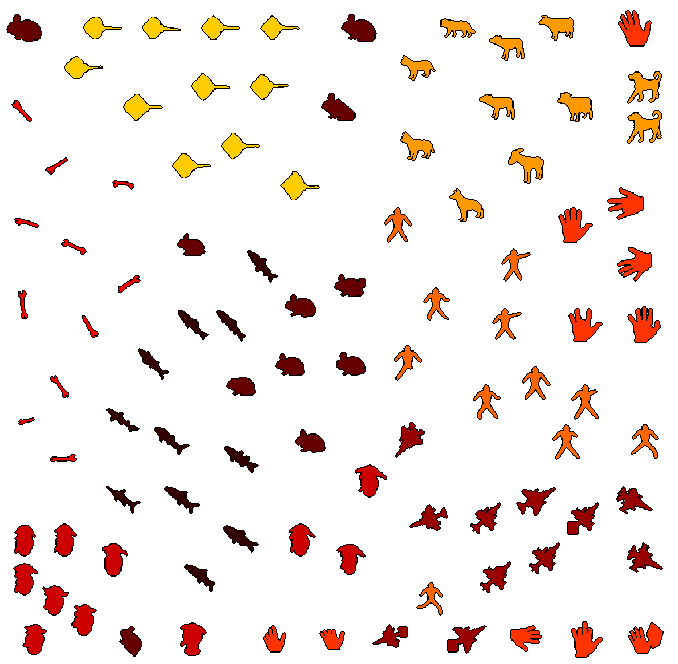
\includegraphics[width=0.5\textwidth]{mapa_som_descritor_dfm.png}
\end{figure}
\end{comment}

\section{Recuperação de imagens pelo conteúdo}

\begin{table*}
\centering
\caption{\label{tab:KimiaChernoff} Total de acertos por classe e por posição, nos experimentos \emph{CBIR}, com a distância de Chernoff.}
\begin{tabular}{l| r r r r r r r r r r r}
\hline
&\multicolumn{11}{l}{nth nearest match} \\
\cline{2-12}
Classe&1&2&3&4&5&6&7&8&9&10&11 \\
 \hline
Peixes&11&11&11&11&9&5&8&3&7&5&5\\
Coelhos&11&11&11&11&11&11&11&11&11&11&7\\ 
Aviões&11&10&8&8&7&7&7&5&2&1&1\\
ETs&11&11&11&11&11&11&11&11&8&7&5\\
Ferramentas&11&8&7&10&3&9&9&5&7&9&9\\
Mãos&11&11&11&11&11&11&11&11&11&9&7\\
humanos&11&11&11&11&11&11&11&11&11&11&11\\
Quadrupedes&11&11&9&8&8&7&8&3&5&8&4\\
Arraias&11&11&11&11&11&11&11&10&11&9&7\\
\hline
Total&99&95&90&92&82&83&87&70&73&70&56\\
\hline
\end{tabular}
\end{table*}

\begin{table*}
\centering
\caption{\label{tab:KimiaChi-square} Total de acertos por classe e por posição, nos experimentos \emph{CBIR}, com a distância de Chi-square.}
\begin{tabular}{l| r r r r r r r r r r r}
\hline
&\multicolumn{11}{l}{nth nearest match} \\
\cline{2-12}
Classe&1&2&3&4&5&6&7&8&9&10&11 \\
 \hline
Peixes&11&11&11&10&10&8&7&9&4&4&3\\
Coelhos&11&10&10&10&10&10&10&10&10&8&1\\ 
Aviões&11&11&11&9&9&9&8&5&2&2&2\\
ETs&11&11&11&10&11&10&11&10&10&8&7\\
Ferramentas&11&11&11&11&11&11&11&11&10&11& 11\\
Mãos&11&11&11&11&11&11&11&11&11&11&9\\
humanos&11&11&11&11&11&11&11&11&11&11&11\\
Quadrupedes&11&11&6&9&8&7&7&5&7&7&4\\
Arraias&11&11&11&11&11&11&11&10&11&11&10\\
\hline
Total&99&98&93&92&92&88&87&82&76&73&58\\
\hline
\end{tabular}
\end{table*}

\begin{table*}
\centering
\caption{\label{tab:KimiaHellinger} Total de acertos por classe e por posição, nos experimentos \emph{CBIR}, com a distância de Hellinger.}
\begin{tabular}{l| r r r r r r r r r r r}
\hline
&\multicolumn{11}{l}{nth nearest match} \\
\cline{2-12}
Classe&1&2&3&4&5&6&7&8&9&10&11 \\
 \hline
Peixes&11&11&11&10&10&9&5&8&8&2&2\\
Coelhos&11&11&11&11&11&10&10&10&11&8&2\\ 
Aviões&11&11&11&10&9&11&9&8&1&1&0\\
ETs&11&11&11&11&10&11&10&11&11&7&4\\
Ferramentas&11&11&11&11&11&11&11&10&11&11& 10\\
Mãos&11&11&11&11&11&11&11&11&11&11&8\\
humanos&11&11&11&11&11&11&11&11&11&11&11\\
Quadrupedes&11&11&7&9&6&6&5&7&9&5&4\\
Arraias&11&11&11&11&11&11&11&11&11&10&9\\
\hline
Total&99&99&95&95&90&91&83&87&84&66&50\\
\hline
\end{tabular}
\end{table*}

\begin{table*}
\centering
\caption{\label{tab:KimiaJensen-Shannon} Total de acertos por classe e por posição, nos experimentos \emph{CBIR}, com a distância Jensen-Shannon.}
\begin{tabular}{l| r r r r r r r r r r r}
\hline
&\multicolumn{11}{l}{nth nearest match} \\
\cline{2-12}
Classe&1&2&3&4&5&6&7&8&9&10&11 \\
 \hline
Peixes&11&11&11&10&10&8&7&7&7&4&1\\
Coelhos&11&10&10&10&10&10&10&10&9&8&2\\ 
Aviões&11&11&10&10&9&8&8&6&3&1&1\\
ETs&11&11&11&10&11&10&10&11&9&8&5\\
Ferramentas&11&11&11&11&11&11&11&11&10&11& 11\\
Mãos&11&11&11&11&11&11&11&11&11&11&9\\
humanos&11&11&11&11&11&11&11&11&11&11&11\\
Quadrupedes&11&11&7&8&8&5&3&8&8&7&4\\
Arraias&11&11&11&11&11&11&11&11&10&11&10\\
\hline
Total&99&98&93&92&92&85&82&86&78&72&54\\
\hline
\end{tabular}
\end{table*}

\begin{table*}
\centering
\caption{\label{tab:KimiaPatrick-Fisher} Total de acertos por classe e por posição, nos experimentos \emph{CBIR}, com a distância Patrick-Fisher.}
\begin{tabular}{l| r r r r r r r r r r r}
\hline
&\multicolumn{11}{l}{nth nearest match} \\
\cline{2-12}
Classe&1&2&3&4&5&6&7&8&9&10&11 \\
 \hline
Peixes&11&11&11&10&10&9&8&5&4&1&1\\
Coelhos&11&9&9&9&9&10&10&9&7&4&4\\ 
Aviões&11&11&10&9&8&9&7&5&3&2&2\\
ETs&11&11&11&10&9&9&9&9&7&6&5\\
Ferramentas&11&10&11&11&11&10&11&11&7&9  &7\\
Mãos&11&11&11&11&11&11&11&11&11&11&9\\
humanos&11&11&11&11&11&11&11&11&11&11&10\\
Quadrupedes&11&11&8&9&8&7&5&5&7&6&6\\
Arraias&11&11&11&11&11&11&10&10&11&9&6\\
\hline
Total&99&96&93&91&88&87&82&76&68&59&50\\
\hline
\end{tabular}
\end{table*}


\begin{figure}[h!]
  \caption{\label{fig:graph1} Gráficos precisão/revocação para diferentes combinações de assinaturas. Resultados obtidos nos experimentos de recuperação de formas pelo conteúdo, com a base de imagens MPEG-7, empregando como medida de similaridade o divergente de Hellinger. }
  \centering
  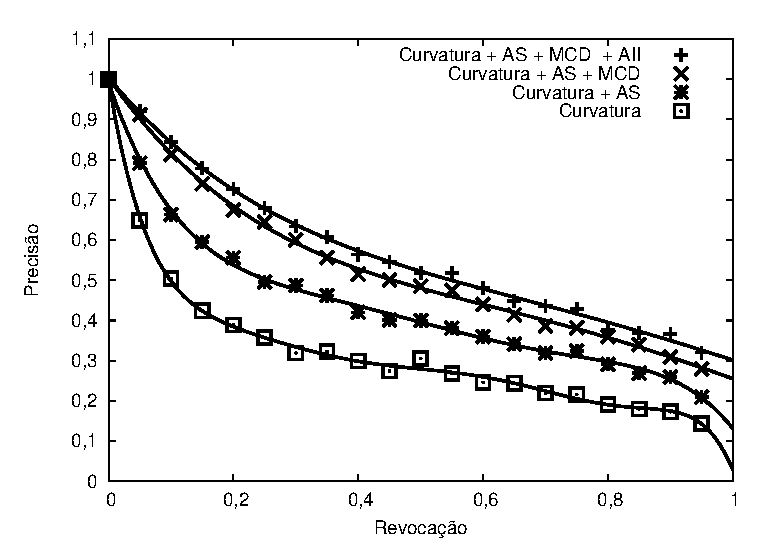
\includegraphics[width=0.75\textwidth]{graph1.eps}
\end{figure}


\begin{comment}
\section{\emph{Gap semântico}}
Uma questão importante nos sistemas \emph{CBIR} é que, embora os usuários busquem por imagens similares do ponto de vista semântico, o sistema provê os resultados com base na similaridade da informação extraída do conteúdo visual das imagens. A disparidade existente entre esses aspectos (semântica e conteúdo visual) é denominado de \emph{Gap} semântico.

Embora as imagens transmitam determinadas mensagens ao usuário, muito frequentemente os atributos extraídos das mesmas não conseguem representar e caracterizar essas mensagens. Diversos métodos para associar informação semântica aos atributos extraídos das imagens têm sido foco de pesquisa, como por exemplo solicitar que o usuário retro-alimente o sistema com o grau de relevância dos resultados obtidos (relevance feedback). 

\section{Base de imagens}

Um aspecto importante em \emph{CBIR} está ligado ao mecanismo de indexação empregado no acesso a informação contida na base de imagens. Em aplicações práticas, que requerem acesso a uma extensa base de dados, e aonde há interação dos usuários com o mecanismo de busca, o desempenho computacional no processo de indexação não pode ser negligenciado. Desta forma, armazenar vetores de características em um arquivo linear, com um registro para cada vetor, resulta na indexação sequencial destes elementos tornando essa abordagem inviável.

Todavia, mecanismos alternativos de indexação tradicionalmente encontrados na literatura, tais como \emph{k-d-b tree}, \emph{quad-tree} e \emph{R-tree} são considerados inadequados em \emph{CBIR} porque o desempenho destes se degrada substancialmente com o aumento da dimensionalidade dos dados. Ademais, para alcançar a eficiência computacional requerida sem degradar a qualidade das buscas, tais mecanismos devem levar em consideração a representação das características das imagens no processo de recuperação, ou seja, não só apenas \emph{como} indexar elementos na base de dados, mas também \emph{o que} indexar.

\end{comment}
